
%%%%%%%%%%%%%%%%%%%%%%%%%%%%%%%%%%%%%%%%%%%%%%%%%%%%%%%%%%%%%%%%%%%%%%
%%%%                   Complex
%%%%%%%%%%%%%%%%%%%%%%%%%%%%%%%%%%%%%%%%%%%%%%%%%%%%%%%%%%%%%%%%%%%%%%

\subsection{Glyph: \glyph{Complex}}\label{sec:complex}

A \glyph{complex} node represents a biochemical entity composed of other biochemical entities, whether macromolecules, simple chemicals, multimers, or other complexes. The resulting entity may have its own identity, properties and function in an SBGN map. A \glyph{complex} possesses its own container box surrounding the juxtaposed container boxes of its components.  This container box is a rectangle with cut-corners (an octagonal box with sides of two different lengths).  The size of the cut-corners are adjusted so that there is no overlap between the container and the components.  The container boxes of the components must not overlap.

\begin{figure}[H]
  \centering
  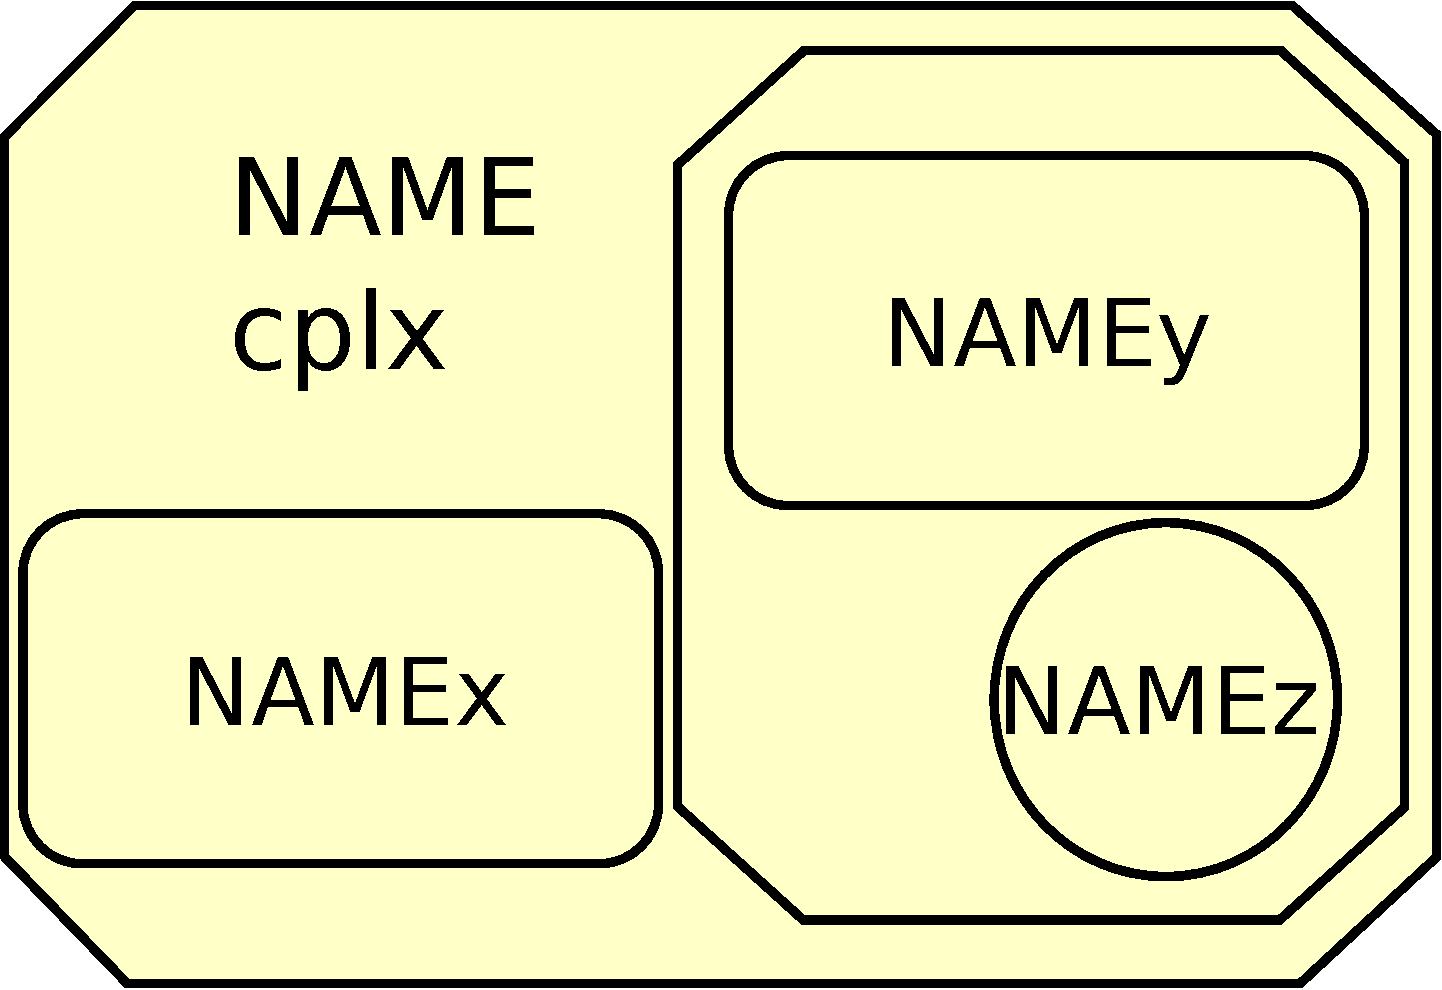
\includegraphics[scale = 0.3]{images/complex}
  \caption{The \PD glyph for \glyph{complex}.}
  \label{fig:complex}
\end{figure}


Examples of \glyph{complexes} are presented in \fig{complex-examples}.

\begin{figure}[H]
  \centering
  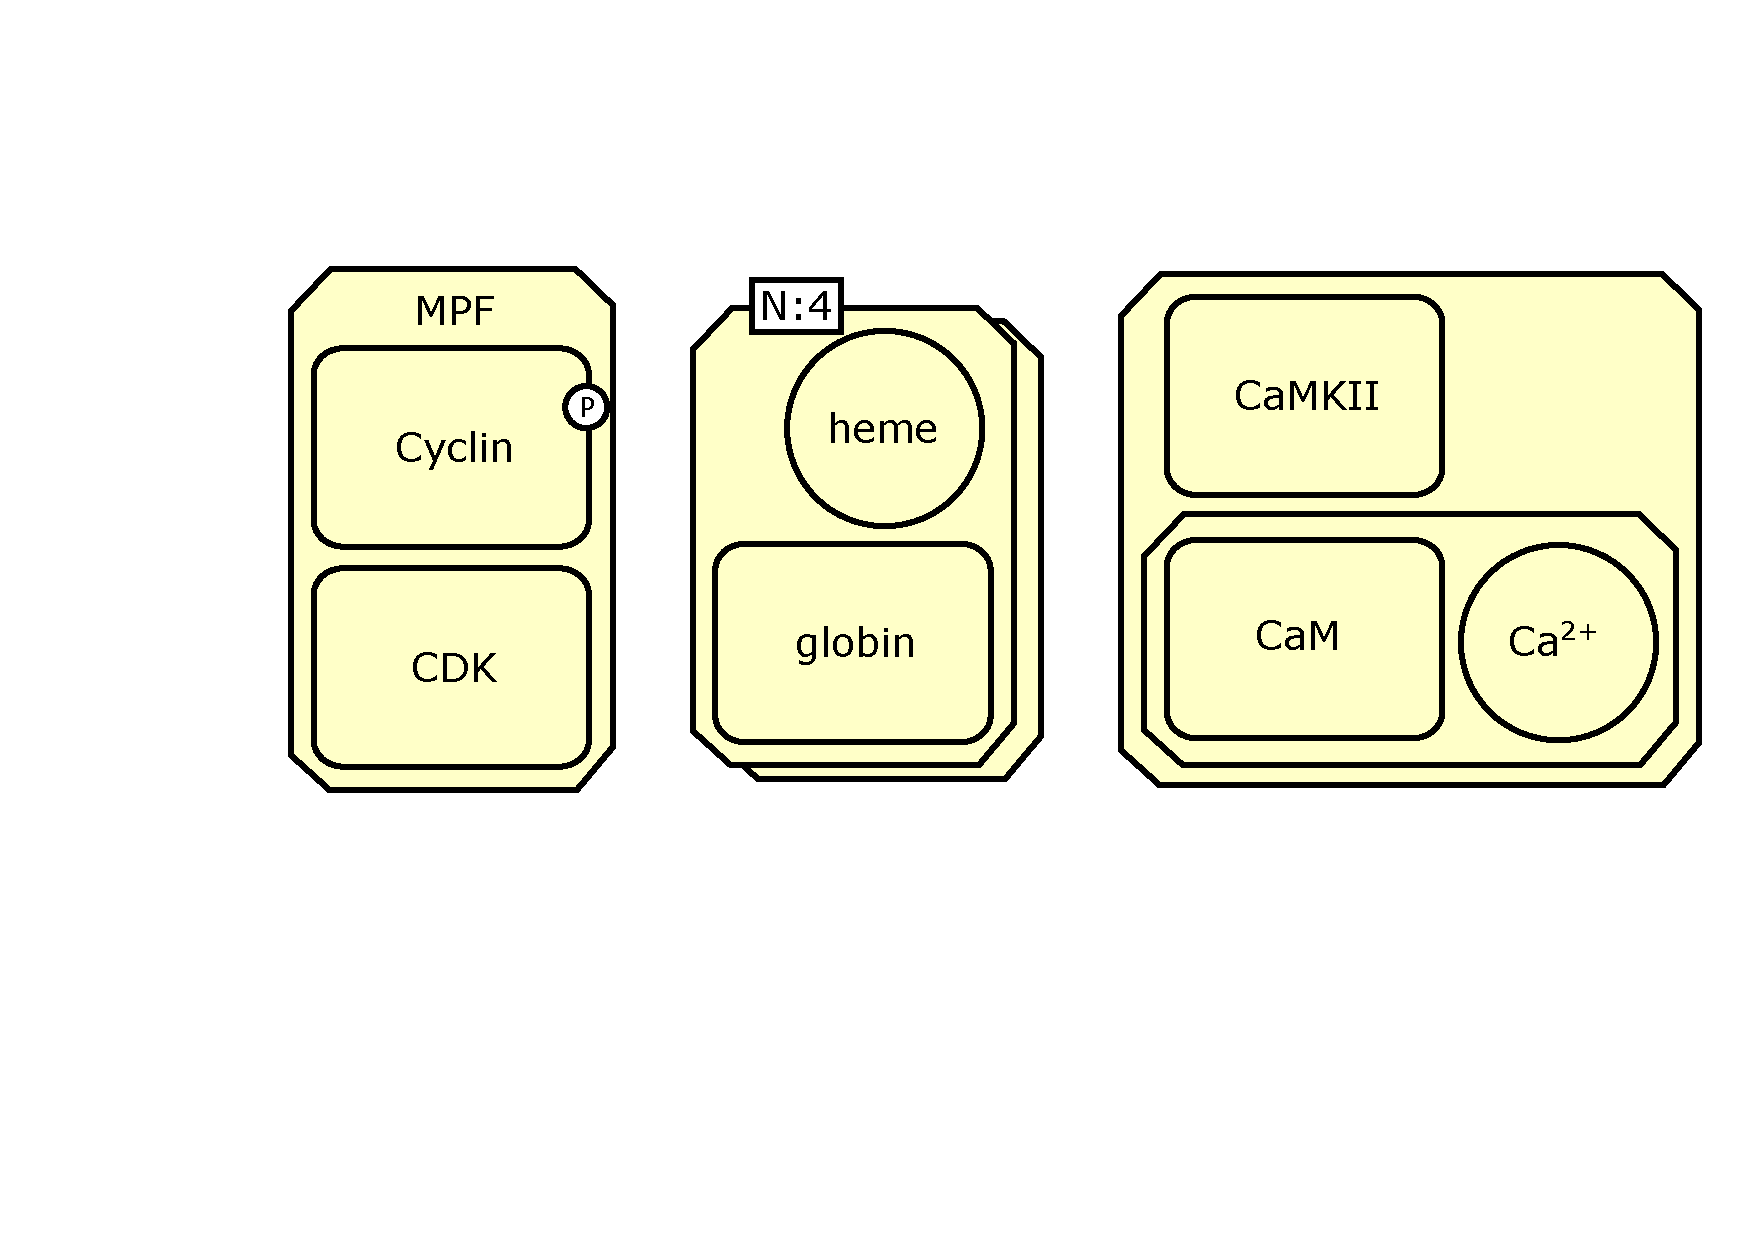
\includegraphics[scale = 0.5]{images/complex-examples}
  \caption{Examples of \glyph{complexes}. From left to right: complex between phosphorylated cyclin and CDK2 forming the maturation promoting factor in yeast, a tetramer of complexes between globin and heme, and a complex between calcium-calmodulin kinase II and another complex, itself formed of calmodulin and calcium.}
  \label{fig:complex-examples}
\end{figure}
